\section{Introduction}

% \begin{figure}[H]
%   \centering
% 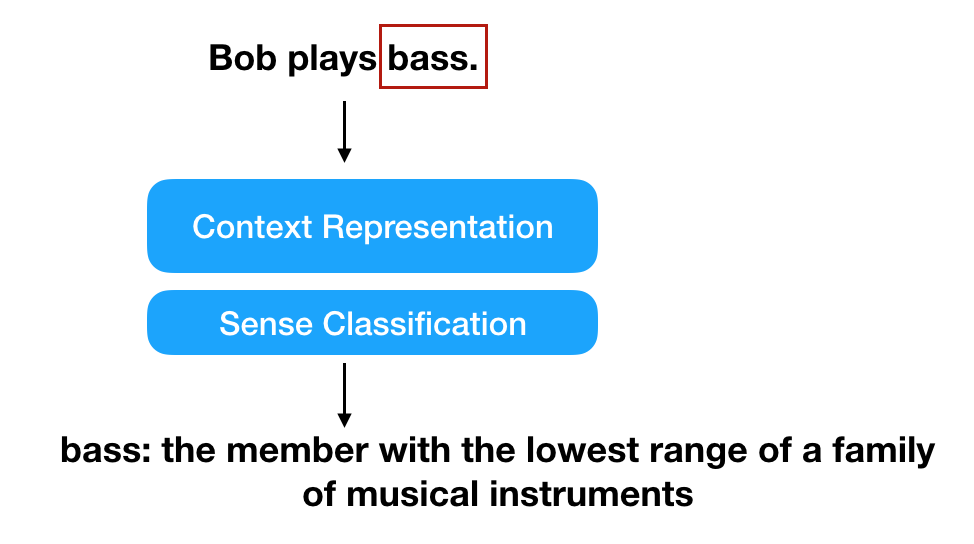
\includegraphics[width=0.5\textwidth]{graphs/overview.png}
% \caption{system overview}
%   \label{fig:overview}
% \end{figure}
% 
Words in natural language could have multiple meanings. Though humans are good
at inducing the actual meaning of words given a certain context, such
multi-meaning words are often seem ambiguous to machines. Such ambiguiaty in
natural languages have been the major challenges for machine to understand user
intention, e.g. google search key words.

To solve this problem, we propose to build a word sense disambiguate system that
takes an English word and a sentence where it appears as input, and predicts the
sense of such word within the given context. 
% The architecture of our system is shown in figure~\ref{fig:overview}.
